\chapter{Background}
Navigation of mobile robots in complex environments has always been a critical topic in the field of robotics research. Such environments often involve static and dynamic obstacles, uneven terrain, and various operational uncertainties. To address these challenges, numerous efficient navigation algorithms have been developed worldwide, finding applications across industries such as industrial automation, autonomous transportation, and surveillance. In this chapter, I will introduce some classical navigation algorithms.

The classical VO method, proposed by Fiorini and Shiller, determines safe trajectories by analyzing the relative velocities between obstacles and the robot \cite{Fiorini1998}, provides a foundation for dynamic collision avoidance in 2D spaces. Recent advances extend this method to three-dimensional scenarios, allowing safe navigation of unmanned aerial vehicles in cluttered airspaces \cite{Bareiss2015}.

Model Predictive Control (MPC) has emerged as a highly effective strategy. By continuously optimizing control inputs over a finite horizon, MPC facilitates real-time trajectory planning while ensuring stability \cite{Mayne2014}. Approaches like Tube MPC, which fall under robust MPC strategies, are well-suited for uncertain environments due to their ability to incorporate error bounds, ensuring the maintenance of stable and reliable trajectories \cite{Mayne2014}.

The Artificial Potential Field (APF) method is a popular reactive navigation technique that uses a virtual field to guide robots toward their targets. In this field, obstacles generate repelling forces, while the target exerts an attractive force \cite{Kim2000}. Enhancing its practical use, researchers have incorporated kinematic constraints, making it more suitable for real-world robotic applications \cite{Ge2000}.

The Bug algorithm is also a strategy for navigation in unknown environments. These algorithms rely on local sensing to avoid obstacles while ensuring progress toward the goal. Their simplicity and guaranteed convergence make them ideal for robots with limited computational resources \cite{Lumelsky1991}. The classic Bug1 and Bug2 algorithms have been enhanced to improve efficiency and adaptability in dynamic and cluttered settings \cite{Lumelsky1991}.

In multirobot systems, coordination becomes critical for efficient and collision-free operation. Distributed MPC has emerged as a promising approach, enabling robots to optimize their trajectories collaboratively while taking into account the constraints of other robots in the environment \cite{Turpin2014}. Furthermore, augmented Lagrangian decomposition techniques have been employed to achieve scalable decentralized navigation in large robotic teams \cite{Dunbar2006}.

 A comprehensive comparison of these algorithms is presented in a table from the work of Hoy, Matveev, and Savkin \cite{Hoy2015}, which categorizes different methods based on their applicability to specific scenarios such as single vehicle navigation, avoidance of moving obstacles, coordination of multiple vehicles, and boundary following.

 \begin{figure}[H]
    \centering
    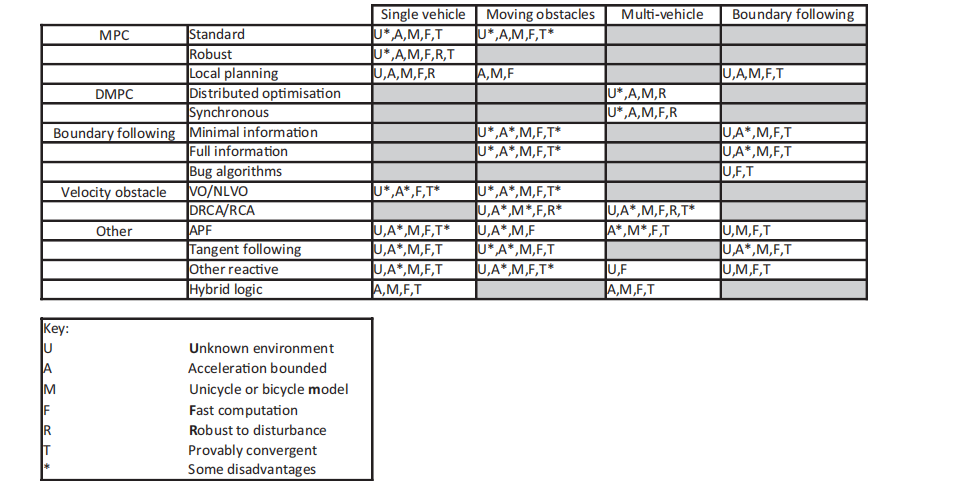
\includegraphics[width=0.8\textwidth]{11.png}
    \caption{compares the applicability of various algorithms discussed in \cite{Hoy2015}}
    \label{FIG:11}
\end{figure}

This paper focuses on discussing the operational strategy of the Sliding Mode Control (SMC) method and testing its performance in various obstacle scenarios. The strategy will be evaluated at the end of the paper.